% Figure 1 (v26): three evaluation confounds that a final-state score cannot distinguish.
% pdfLaTeX + TikZ + Libertine; counts from the archived replay outputs (see v25 data notes).
\documentclass[border=0pt]{standalone}
\usepackage[T1]{fontenc}
\usepackage{libertine}
\usepackage{tikz}
\usetikzlibrary{patterns}
\definecolor{agreeG}{rgb}{0.54118,0.56471,0.60000}
\definecolor{allowG}{rgb}{0.78824,0.80392,0.82745}
\definecolor{litB}{rgb}{0.56078,0.72550,0.92549}
\definecolor{witB}{rgb}{0.16472,0.47060,0.83922}
\definecolor{remO}{rgb}{0.92157,0.40784,0.20392}
\definecolor{muted}{HTML}{6B6A66}
\newcommand{\ttl}[1]{\fontsize{8.4}{10.4}\selectfont\bfseries #1}
\newcommand{\sm}{\fontsize{7.6}{9.6}\selectfont}
\newcommand{\xs}{\fontsize{7}{8.4}\selectfont}
\begin{document}
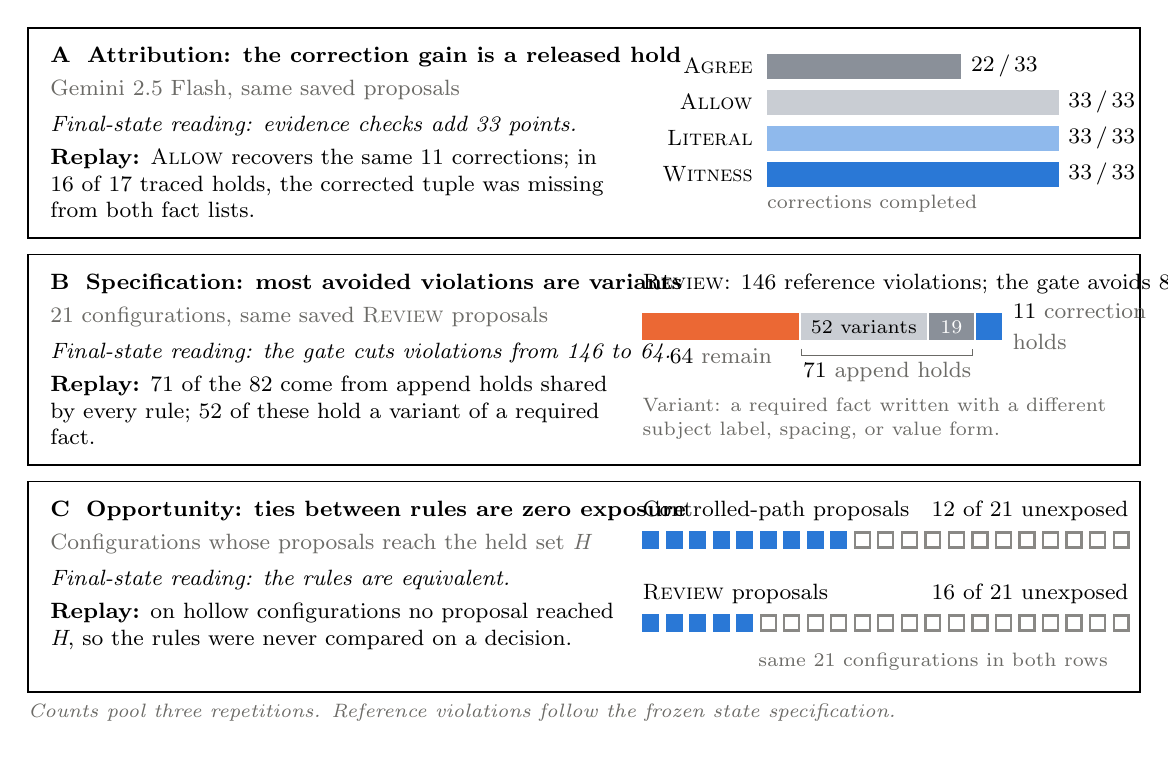
\begin{tikzpicture}[x=1pt,y=-1pt,every node/.style={inner sep=0pt,outer sep=0pt}]
\path[use as bounding box] (0,0) rectangle (402,256);
% ---------- frames
\foreach \y in {0,82,164} \draw[line width=.6pt] (0,\y) rectangle (402,\y+76);
% ---------- left text, shared style
\newcommand{\panel}[6]{%
 \node[anchor=north west] at (8.2,#1+7) {\ttl{#2\hspace{.6em}#3}};
 \node[anchor=north west,text=muted] at (8.2,#1+19) {\sm #4};
 \node[anchor=north west] at (8.2,#1+32) {\sm\itshape #5};
 \node[anchor=north west,text width=206pt,align=flush left,font=\sm] at (8.2,#1+44) {\textbf{Replay:} #6};}
\panel{0}{A}{Attribution: the correction gain is a released hold}{Gemini 2.5 Flash, same saved proposals}
 {Final-state reading: evidence checks add 33 points.}
 {\textsc{Allow} recovers the same 11 corrections; in 16 of 17 traced holds, the corrected tuple was missing from both fact lists.}
\panel{82}{B}{Specification: most avoided violations are variants}{21 configurations, same saved \textsc{Review} proposals}
 {Final-state reading: the gate cuts violations from 146 to 64.}
 {71 of the 82 come from append holds shared by every rule; 52 of these hold a variant of a required fact.}
\panel{164}{C}{Opportunity: ties between rules are zero exposure}{Configurations whose proposals reach the held set \textit{H}}
 {Final-state reading: the rules are equivalent.}
 {on hollow configurations no proposal reached \textit{H}, so the rules were never compared on a decision.}
% ---------- A: bars (scale 105.6pt = 33)
\def\sc{3.2}
\foreach \lab/\val/\col/\yy in {Agree/22/agreeG/9.5, Allow/33/allowG/22.5, Literal/33/litB/35.5, Witness/33/witB/48.5}{
 \node[anchor=east] at (262,\yy+4.5) {\sm\textsc{\lab}};
 \fill[\col] (267,\yy) rectangle ({267+\val*\sc},\yy+9);
 \node[anchor=west] at ({267+\val*\sc+3.5},\yy+4.5) {\sm \val\,/\,33};}
\node[anchor=north west,text=muted] at (267.2,60.5) {\xs corrections completed};
% ---------- B: stacked bar, 146 total over 130pt
\def\u{0.89041}
\node[anchor=north west] at (222.2,89) {\sm\textsc{Review}: 146 reference violations; the gate avoids 82};
\fill[remO]  (222,103) rectangle ({222+64*\u},113);
\fill[allowG] ({222+64*\u},103) rectangle ({222+116*\u},113);
\fill[agreeG] ({222+116*\u},103) rectangle ({222+135*\u},113);
\fill[witB]  ({222+135*\u},103) rectangle ({222+146*\u},113);
\draw[white,line width=.8pt] ({222+64*\u},103) -- ({222+64*\u},113) ({222+135*\u},103) -- ({222+135*\u},113);
\draw[white,line width=.5pt] ({222+116*\u},103) -- ({222+116*\u},113);
\node at ({222+90*\u},108.2) {\xs 52 variants};
\node[text=white] at ({222+125.5*\u},108.2) {\xs 19};
\node[anchor=west,align=left] at ({222+146*\u+4},108) {\sm 11 \textcolor{muted}{correction}\\[-1pt]\sm\textcolor{muted}{holds}};
% labels below
\node[anchor=north] at ({222+32*\u},116) {\sm 64 \textcolor{muted}{remain}};
\draw[muted,line width=.4pt] ({222+64.8*\u},116) -- ({222+64.8*\u},118.5) -- ({222+134.2*\u},118.5) -- ({222+134.2*\u},116);
\node[anchor=north] at ({222+99.5*\u},121) {\sm 71 \textcolor{muted}{append holds}};
\node[anchor=north west,text=muted,text width=172pt,align=flush left,font=\xs] at (222.2,134) {Variant: a required fact written with a different subject label, spacing, or value form.};
% ---------- C: exposure squares (21 per row, step 8.5pt)
\newcommand{\squares}[2]{% #1 = y, #2 = exposed count
 \foreach \i in {0,...,20}{
  \pgfmathsetmacro{\xx}{222+\i*8.5}
  \ifnum\i<#2 \fill[witB] (\xx,#1) rectangle (\xx+6.2,#1+6.2);
  \else \draw[muted!80,line width=.8pt] (\xx+.4,#1+.4) rectangle (\xx+5.8,#1+5.8);\fi}}
\node[anchor=north west] at (222.2,171) {\sm Controlled-path proposals};
\node[anchor=north east] at (397.8,171) {\sm 12 of 21 unexposed};
\squares{182}{9}
\node[anchor=north west] at (222.2,201) {\sm \textsc{Review} proposals};
\node[anchor=north east] at (397.8,201) {\sm 16 of 21 unexposed};
\squares{212}{5}
\node[anchor=north west,text=muted] at (264,226) {\xs same 21 configurations in both rows};
% ---------- footnote
\node[anchor=north west,text=muted] at (0.2,244.5) {\fontsize{7.2}{8}\selectfont\itshape Counts pool three repetitions. Reference violations follow the frozen state specification.};
\end{tikzpicture}
\end{document}
